\section{Electrical Design}
This section describes the electrical design of the Fixed and Variable Pitch Quadcopters.

\subsection{Schematic}
In Fig. \ref{fig:fpqsch} the schematic for the FPQ is displayed. This diagram is designed based on the DJI E600 motors. 
\begin{figure}[H]
    \centering
    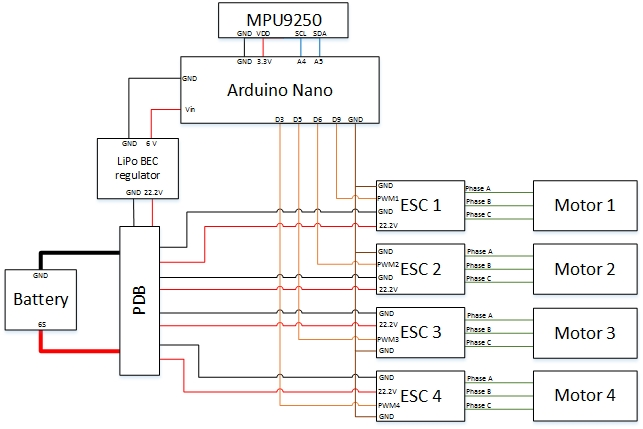
\includegraphics[width = 1\textwidth]{VAPIQ-PICTURES/ShematicFPQ}
    \caption{Schematic for FPQ}
    \label{fig:fpqsch}
\end{figure}
\newpage
\noindent
In Fig. \ref{fig:vpqsch} the schematic for the FPQ is displayed. This diagram is designed based on the AXI 2208/26 motors. 
\begin{figure}[H]
    \centering
    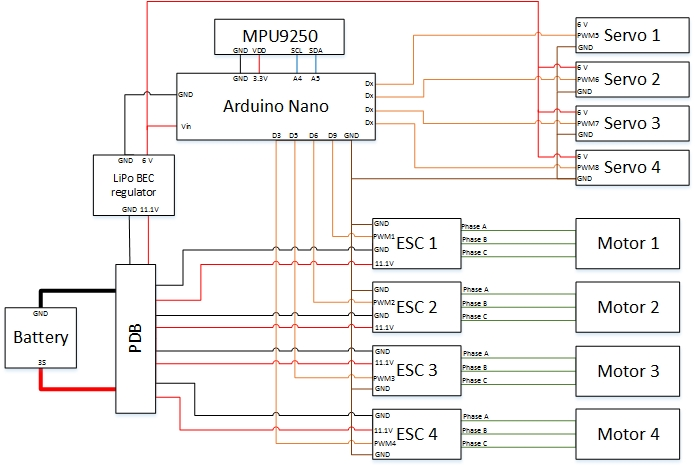
\includegraphics[width = 1\textwidth]{VAPIQ-PICTURES/ShematicVPQ}
    \caption{Schematic for VPQ}
    \label{fig:vpqsch}
\end{figure}
\newpage
\subsection{Components}
In Tab. \ref{tab:CompFPQ} the electrical components needed to construct the FPQ are displayed. This table is designed based on the DJI E600 motors. 
\begin{table}[H]
    \begin{center}
    \caption{Components used for FPQ} 
    \label{tab:CompFPQ} 
        \begin{tabular}{|l|l|c|}
            \hline 
            \textbf{Component:} & \textbf{Info:} & \textbf{Qty.:}  \\ 
            \hline
            Motor & DJI E600  & 4 \\
            ESC & E600 20A & 4 \\
            Bluetooth Module & HC-06 & 1  \\
            Microcontroller & Arduino Nano  ATmega328P& 1 \\
            LiPo Battery & Gens ace 4600mAh, 6S, 35C & 1 \\
            LiPo BEC Regulator & In: 6v-25v, Out: 6V (Max. 5A)  & 1\\
            IMU & MPU9250 & 1 \\
            \hline
        \end{tabular}
    \end{center}
\end{table}
\noindent
To be able to compute the required thrust to hover, the total mass needs to be calculated. In Tab. \ref{tab:WeightFPQ} the mass budget for FPQ is displayed.
\begin{table}[H]
    \begin{center}
    \caption{Mass budget FPQ} 
    \label{tab:WeightFPQ} 
        \begin{tabular}{|l|c|c|}
            \hline 
            \textbf{Component:} & \textbf{Qty.:} & \textbf{Mass[g]:}  \\ 
            \hline
            Frame + cables & 1 & 611.2\\
            Propellers & 4 & 82.8\\
            DJI E600  & 4 & 360 \\
            E600 20A ESC & 4 & 80 \\
            Bluetooth Module HC-06 & 1 & 2\\
            MPU 9250 & 1 & 2 \\
            Arduino Nano & 1 & 7 \\
            LiPo Battery & 1 & 670 \\
            LiPo BEC Regulator & 1 & 19 \\
            PDB & 1 & 20 \\\hline
            \textbf{Total mass budget:} & & 1856\\
            \hline
        \end{tabular}
    \end{center}
\end{table}
\noindent
In Tab. \ref{tab:CompVPQ} the electrical components needed to construct the VPQ are displayed. This table is designed based on the AXI 2208/26 motors. 
\begin{table}[H]
    \begin{center}
    \caption{Components used for VPQ} 
    \label{tab:CompVPQ} 
        \begin{tabular}{|l|l|c|}
            \hline 
            \textbf{Component:} & \textbf{Info:} & \textbf{Qty.:}  \\ 
            \hline
            Motor & AXI 2208/26 Gold Line & 4 \\
            ESC & Turnigy Opto 12A & 4 \\
            Servo & MG90D, 2.4kg\@6V & 4  \\ 
            Bluetooth Module & HC-06 & 1  \\
            Microcontroller & Arduino Nano  ATmega328P& 1 \\
            LiPo Battery & Typhon 2200mAh, 3S, 25C & 1 \\
            LiPo BEC Regulator & In: 6v-25v, Out: 6V (Max. 5A)  & 1\\
            IMU & MPU9250 & 1 \\
            \hline
        \end{tabular}
    \end{center}
\end{table}
\noindent
To be able to compute the required thrust to hover, the total mass needs to be calculated. In Tab. \ref{tab:WeightVPQ} the mass budget for VPQ is displayed.
\begin{table}[H]
    \begin{center}
    \caption{Mass budget VPQ} 
    \label{tab:WeightVPQ} 
        \begin{tabular}{|l|c|c|}
            \hline 
            \textbf{Component:} & \textbf{Qty.:} & \textbf{Mass[g]:}  \\ \hline
            Est. Frame + cables & 1 & 250\\
            Propellers & 4 & 60\\
            AXI 2208/26 Gold Line  & 4 & 180 \\
            ESC & 4 & 20\\
            Servo & 4 & 52 \\
            Bluetooth Module HC-06 & 1 & 2\\
            MPU 9250 & 1 & 2 \\
            Arduino Nano & 1 & 7 \\
            LiPo Battery & 1 & 153 \\
            LiPo BEC Regulator & 1 & 19 \\\hline
            \textbf{Total mass budget:} & & 763 \\
            \hline
        \end{tabular}
    \end{center}
\end{table}
\noindent
As seen from Tab. \ref{tab:CompFPQ} and Tab. \ref{tab:CompVPQ}, the only difference in components needed is the servos for the Variable Pitch Quadcopter. 

\newpage
